\documentclass[12pt]{standalone}
\usepackage[english]{babel}
\usepackage[utf8]{inputenc}

\usepackage{comment}
\usepackage{amsmath}
\usepackage{tikz}
\usepackage{circuitikz} % for circuit stuff
\usetikzlibrary{arrows.meta} % for loads
\usepackage{float}
\usetikzlibrary{positioning}
\usetikzlibrary{calc}

% Custom code for generator
\newcommand\ppbb{path picture bounding box}
\tikzset{
  do path picture/.style={%
    path picture={%
      \pgfpointdiff{\pgfpointanchor{\ppbb}{south west}}%
        {\pgfpointanchor{\ppbb}{north east}}%
      \pgfgetlastxy\x\y%
      \tikzset{x=\x/2.5,y=\y/2.5}%
      #1
    }
  },
  sin wave/.style={do path picture={    
    \draw [line cap=round] (-3/4,0)
      sin (-3/8,1/2) cos (0,0) sin (3/8,-1/2) cos (3/4,0);
  }},
	gen/.style={circle, draw=black, thick, minimum width = 2em,sin wave
	},
}

\begin{document}
	
	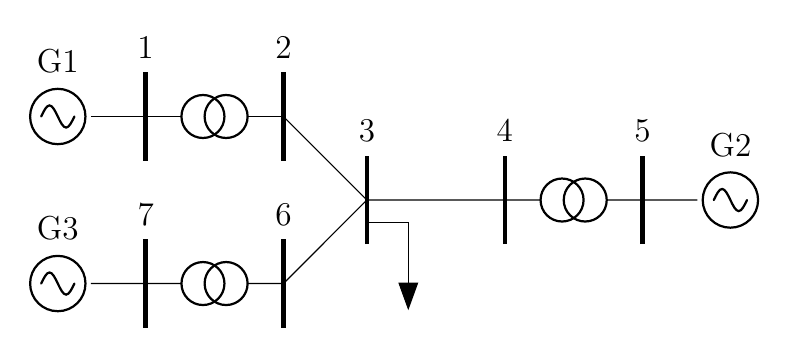
\begin{tikzpicture}[american voltages,
	scale=.7, 
	breaker/.style={rectangle,draw=black,fill=white},
	load/.style={-{Triangle[length=3.5mm,width=2.5mm,open,fill=black]}},
	node distance = 1.75 cm and 1.75 cm]
	
	% bus coordinate def
	% main row ( 2- 5)
	\node[gen] (G1) at (0,0){}; % gen 1
	\coordinate[right = .75 cm of G1] (B1) {};
	\coordinate[right =  of B1] (B2) {};
	\coordinate[below right = 1.5 cm of B2] (B3) {};
	\coordinate[right =  of B3] (B4) {};
	\coordinate[right =  of B4] (B5) {};
	% Gen 3 branch (6, 7)
	\coordinate[below left= 1.5cm of B3] (B6) {};
	\coordinate[left =  of B6] (B7) {};
	
	% gen 2 and 3
	\node[gen,right= .75 cm of B5] (G2) {}; % gen 2
	\node[gen,left= .75 cm of B7] (G3) {}; % gen 3
	
	% vertical bus lines
	\foreach \a in {1, 2, 3, 4, 5, 6, 7}, 
	\draw[ultra thick] ([yshift=-0.8cm]B\a.south) -- ([yshift=+0.8cm]B\a.north);
	
	% xfmrs
	\draw (B2) to [voosource] (B1){};
	\draw (B7) to [voosource] (B6){};
	\draw (B5) to [voosource] (B4){};
	
	%gen lines
	\newcommand{\genOff}{.6} % to make connecting line on edge of gen
	\draw ($(G1)+(\genOff,0)$) -- (B1){};
	\draw ($(G2)+(-\genOff,0)$) -- (B5){};
	\draw ($(G3)+(\genOff,0)$) -- (B7){};
	
	% lines
	\draw (B6) -- (B3){};
	\draw (B2) -- (B3){};
	\draw (B4) --(B3){};
	
	% load coordinates
	\coordinate (L1) at ($ (+.75,-2 ) + (B3)$) {};
	% load arrow
	\draw[load] ($(B3)+(0,-.4)$) -| (L1) ;
	
	% bus labels above
	\foreach \busNum in {1, 2, 3, 4, 5, 6, 7}
	\draw ($(B\busNum) +(0.0, 1.25)$) node {\large{\busNum}};
	
	% gen labels  above
	\foreach \genNum in {1, 2, 3}
	\draw ($(G\genNum) +(0.0, 1.0)$) node {\large{G\genNum}};

	\end{tikzpicture}
	
\end{document}